%************************************************
\section[A directional tuning map of \textit{Drosophila} elementary motion detectors]{A directional tuning map of Drosophila elementary motion detectors}
\sectionmark{A directional tuning map of Drosophila elementary motion detectors}
\label{sct:manuscript_maisak}
%************************************************

This article characterized the response properties of T4 and T5 cells and quantified their particular contribution to downstream networks and behavior. It was published in \textit{Nature} in August 2013 \citep{Maisak:2013kk} and highlighted in several journals \citep{Masland:2013kv,Gilbert:2013aa,Yonehara:2013aa,Flight:2013aa}.

\paragraph{Summary}
Previous work had shown that combined silencing of bushy T4 and T5 cells renders downstream lobula plate tangential cells insensitive to motion stimuli. Using two-photon imaging, we recorded calcium activity in GAL4-targeted T4 or T5 cells. T4 cells that projected to a specific layer of the lobula plate were sensitive to localized ON motion in one of the four cardinal directions (front-to-back, back-to-front, upward, and downward). The four subtypes of T5 cells, in turn, responded to corresponding OFF motion stimuli. Overall, the two cell arrays could be shown to form a retinotopic, polarity-specific, direction-selective map of visual space. Critically, chiasmatic neurites of T4 and T5 already exhibited strong selectivity. Finally, when blocking T4 or T5 individually, downstream tangential cells lost their sensitivity to ON or OFF motion, respectively, while remaining sensitive to the other polarity. A competitive motion assay confirmed these results in walking behavior, strongly suggesting that only T4 and T5 relay ON and OFF motion signals.

\paragraph{Authors}
Matthew S. Maisak, Juergen Haag (co-first author), Georg Ammer, Etienne Serbe, Matthias Meier, \textbf{Aljoscha Leonhardt}, Tabea Schilling, Armin Bahl, Gerald M. Rubin, Aljoscha Nern, Barry J. Dickson, Dierk F. Reiff, Elisabeth Hopp, and Alexander Borst.

\paragraph{Contributions}
M.S.M. and J.H.\ jointly performed and, together with A.Bo., evaluated all calcium imaging experiments. G.A., E.S.\ and M.M.\ recorded from tangential cells. \textbf{A.L.}, T.S. and A.Ba.\ performed the behavioural experiments. G.R., B.D.\ and A.N.\ generated the driver lines and characterized their expression pattern. D.F.R.\ performed preliminary imaging experiments. E.H.\ helped with programming and developed the PMT shielding for the two-photon microscope. A.Bo.\ designed the study and wrote the manuscript with the help of all authors.

\cleardoublepage

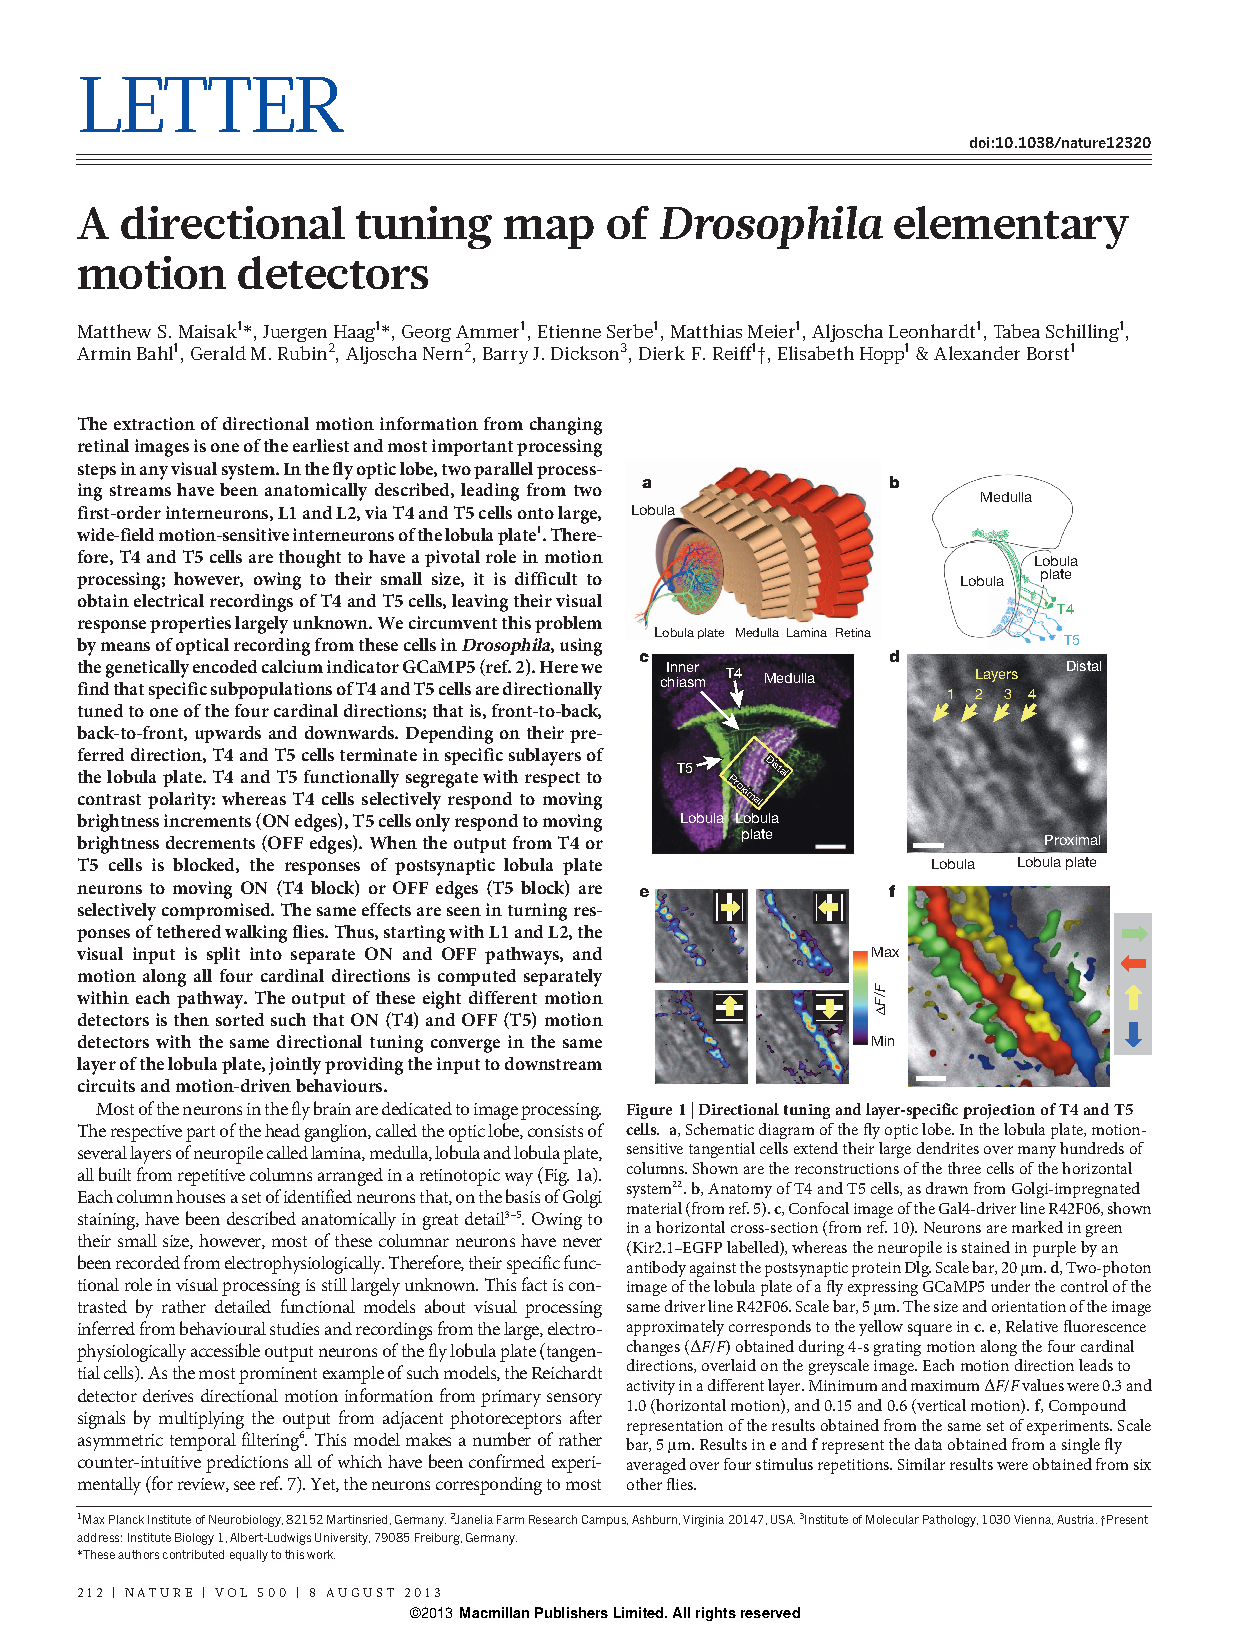
\includepdf[pages=-,scale=0.9,offset= 0 40,pagecommand={\thispagestyle{plain}}]{papers/maisak2013}
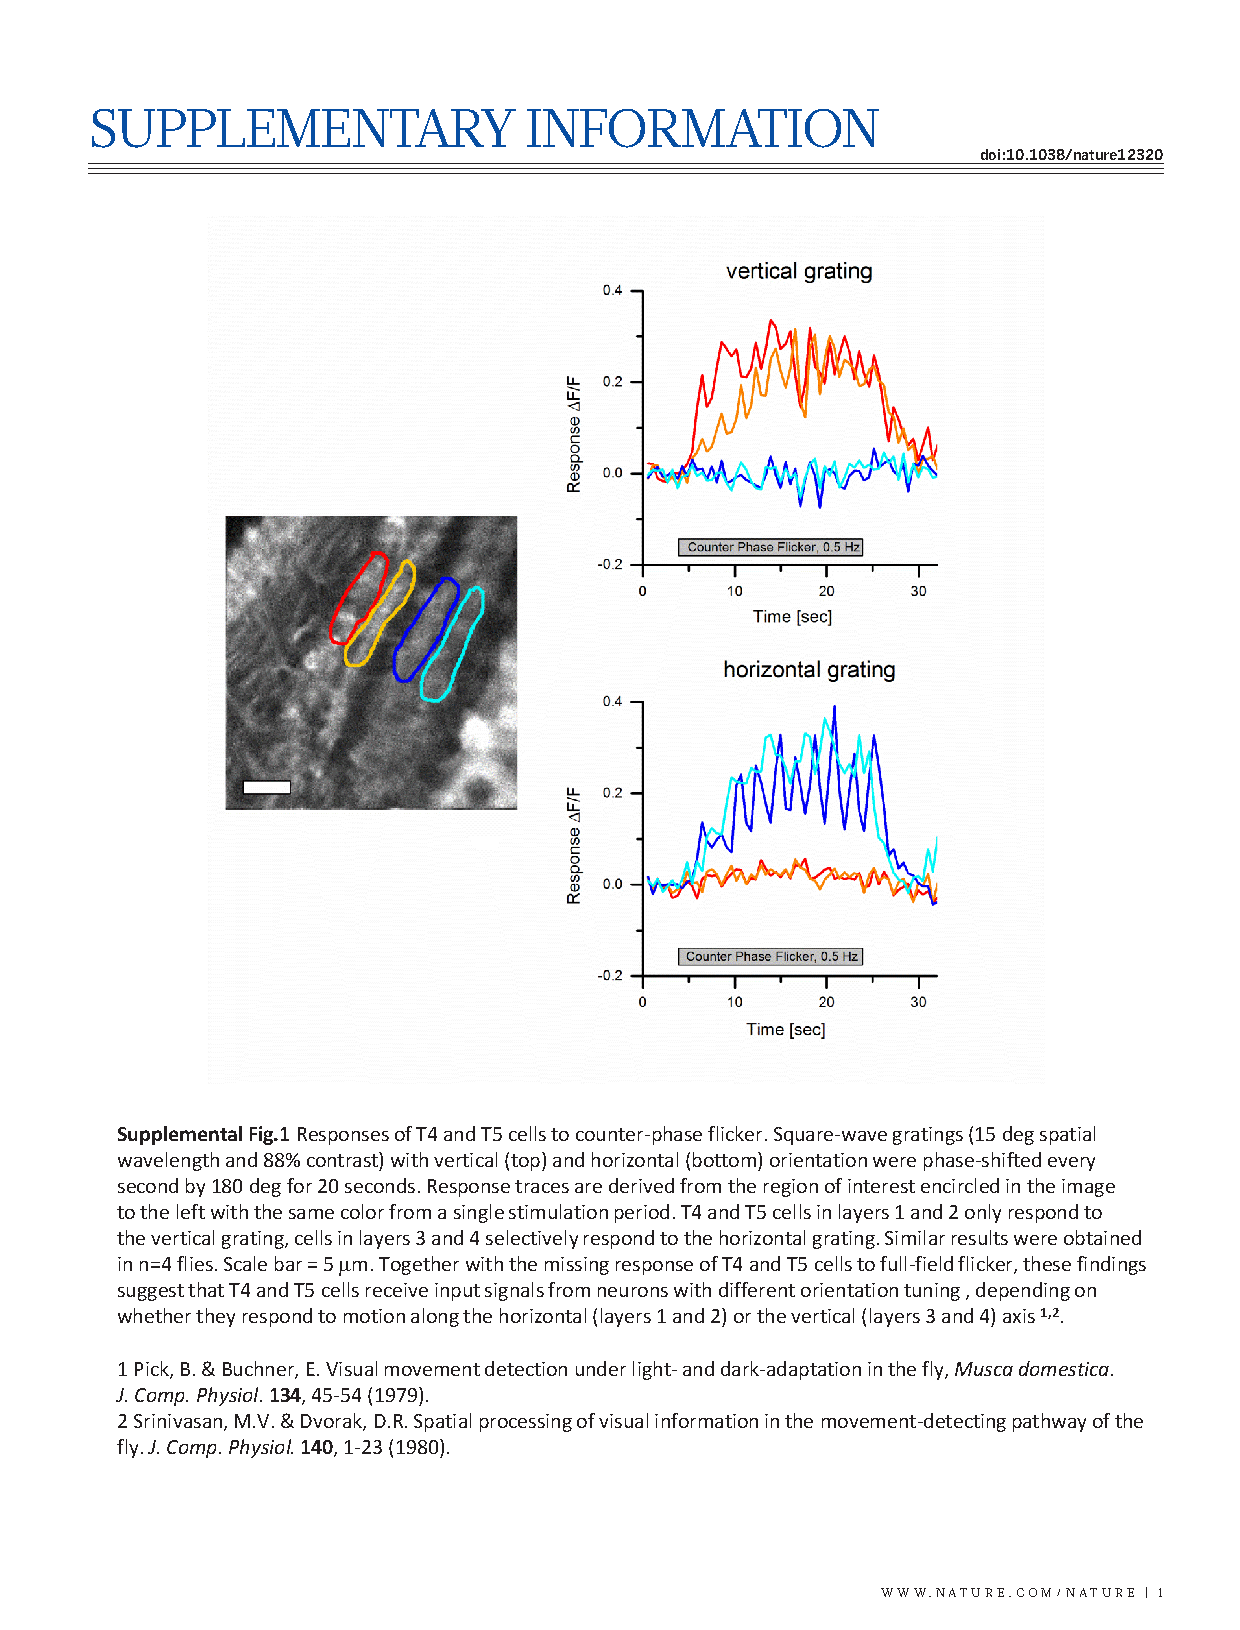
\includepdf[pages=-,scale=0.9,offset= 0 40,pagecommand={\thispagestyle{plain}}]{papers/maisak2013_supplement}